\documentclass[oneside]{fduthesis}

\fdusetup{
  style = {
    font = lm,
    % 西文字体(包括数学字体)
    % 允许选项:
    %   font = garamond|libertinus|lm|palatino|times
    %
    % 注意:
    %   1. LaTeX 默认风格是 lm
    %   2. Satoshi 的讲义风格是 palatino
    %
    cjk-font = windows,
    % 中文字体
    % 允许选项:
    %   cjk-font = adobe|fandol|founder|mac|sinotype|sourcehan|windows
    %
    % 注意:
    %   1. 中文字体设置高度依赖于系统。各系统建议方案:
    %        windows:cjk-font = windows
    %        mac:    cjk-font = mac
    %        linux:  cjk-font = fandol(默认值)
    %   2. 除 fandol 和 sourcehan 外,其余字体均为商用字体,请注意版权问题
    %   3. 但 fandol 字体缺字比较严重,而 sourcehan 没有配备楷体和仿宋体
    %   4. 某些字体会有 Font "xxx" does not contain requested Script "CJK" 的警告,可以忽略
    %
    font-size    = -4,
    bib-backend  = bibtex,
    bib-resource = {main.bib},
  },
  info = {
      title            = {数值Bootstrap及其在凝聚态物理中的应用},
      % title            = {如果标题很长,可以用英文逗号分成两行},
      author           = {吴晋渊},
      department       = {物理学系},
      major            = {物理学},
      supervisor       = {戚扬},
      supervisor-title = {研究员},
      affiliation      = {物理学系},
      student-id       = {18307110155},
      keywords         = {Bootstrap, Hubbard模型, 非线性谐振子},
      keywords*        = {Bootstrap, Hubbard model, nonlinear oscillator},
      % 中英文关键字均使用英文逗号分隔
  }
}

% 需要的宏包可以自行调用
\usepackage{booktabs}
\usepackage{amsmath}
\usepackage{mathtools}
\usepackage{siunitx}
\usepackage{physics}
\usepackage{tikz}
\usepackage{cancel}
\usepackage{color}
\usepackage{array}
\usepackage{multirow}
\usepackage{tabularx}
\usepackage{extarrows}
\usepackage[linkcolor=black,menucolor=black]{hyperref}
\usepackage{prettyref}

\usetikzlibrary{fadings}
\usetikzlibrary{patterns}
\usetikzlibrary{shadows.blur}
\usetikzlibrary{shapes}

\newrefformat{chap}{第\ref{#1}章}
\newrefformat{sec}{第\ref{#1}节}
\newrefformat{note}{注\ref{#1}}
\newrefformat{fig}{图\ref{#1}}
\newrefformat{alg}{算法\ref{#1}}

\newcommand{\hilbertH}{\symcal{H}}
\newcommand{\ee}{\symrm{e}}
\newcommand{\ii}{\symrm{i}}

% Disable unsupported commands in bookmark titles 
\pdfstringdefDisableCommands{%
  \def\\{}%
  \def\texttt#1{<#1>}%
  \def\mathbb#1{#1}%
}
\pdfstringdefDisableCommands{\def\eqref#1{(\ref{#1})}}

\makeatletter
\pdfstringdefDisableCommands{\let\HyPsd@CatcodeWarning\@gobble}
\makeatother

% 图片路径
% \graphicspath{{images/}}

% 目录深度,只保留到 \section
\setcounter{tocdepth}{2}

\begin{document}

% 前置部分包含目录、中英文摘要以及符号表等
\frontmatter

% 目录
\tableofcontents
% 插图目录
%\listoffigures
% 表格目录
% \listoftables

\begin{abstract}
TODO
\end{abstract}

\begin{abstract*}
TODO
\end{abstract*}

% 主体部分是论文的核心
\mainmatter

\ctexset{chapter/pagestyle=fancy}

% 建议采用多文件编译的方式
% 比较好的做法是把每一章放进一个单独的 tex 文件里,并在这里用 \include 导入,例如
%   \include{chapter1}
%   \include{chapter2}
%   \include{chapter3}

\chapter{绪论}

\section{引言}

凝聚态物理分析

\section{Bootstrap技术示例:共形Bootstrap}

最为著名的bootstrap方法可能是所谓的共形bootstrap,即针对共形场论(conformal field theory, CFT)的bootstrap。
共形对称性对两点和三点关联函数的形式有着强烈的要求:关于标量算符$\mathcal{O}$的两点函数只能够取
\begin{equation}
    \expval*{\mathcal{O}(x) \mathcal{O}(y)} = \frac{1}{{\abs*{x - y}}^{2 \Delta_{\mathcal{O}}}}
    \label{eq:two-point-conformal}
\end{equation}
的形式,其中$\Delta_{\mathcal{O}}$是常数(实际上是算符$\mathcal{O}$的反常量纲),而三点函数只能够取
\begin{equation}
    \langle\mathcal{A}(x) \mathcal{B}(y) \mathcal{C}(z)\rangle = \frac{f_{\mathcal{A B C}}}{|x-y|^{\Delta \mathcal{A}+\Delta_{\mathcal{B}}-\Delta_{\mathcal{C}}}|y-z|^{\Delta_{\mathcal{B}}+\Delta_{\mathcal{C}}-\Delta \mathcal{A}}|z-x|^{\Delta_{\mathcal{C}}+\Delta_{\mathcal{A}}-\Delta_{\mathcal{B}}}}
    \label{eq:three-point-conformal}
\end{equation}
的形式。如果$\mathcal{O}$有自旋$l_{\mathcal{O}}$,分子上可能还会出现一些因子。
在已知两点函数和三点函数之后,可以通过算符乘积展开将更高阶的关联函数递归地计算出来。于是,确定一个CFT需要的数据就是$\{\Delta_{\mathcal{O}}, l_{\mathcal{O}}, f_{\mathcal{A} \mathcal{B} \mathcal{C}}\}$。
我们随后可以通过一系列约束条件,获得关于这些数据的不等式,从而确定自洽的CFT的$\{\Delta_{\mathcal{O}}, l_{\mathcal{O}}, f_{\mathcal{A} \mathcal{B} \mathcal{C}}\}$组合。
通过这种方式,在给定一类CFT的基本自由度之后,我们实际上已经知道这整整一类CFT的行为以及理论空间的边界了\cite{Poland_2016,2019}。

在凝聚态物理中,$1+1$维无能隙体系常常可以使用CFT描述,如Luttinger液体及其推广,如霍尔效应边界态\cite{Degiovanni_1998}。
共形bootstrap可以为一个体系的临界行为是不是能够使用CFT描述提供一定提示,如通过比较三维伊辛模型和一类CFT的临界指数,我们有很强的信心表明三维伊辛模型的临界行为可能就是一个落在可行域边界上的CFT\cite{prd2012ising,Poland_2016}。

\section{数值bootstrap}

\subsection{形式理论}

实际问题中会遇到的模型大多不像CFT那样容易做bootstrap:我们没有像\eqref{eq:two-point-conformal}和
\eqref{eq:three-point-conformal}这么强的对关联函数的约束条件,一般情况下也不能解析地将高阶关联函数转化为低阶关联函数的多项式。
然而,这不意味着bootstrap的思想和一些计算手段不能够适用于非CFT的体系:我们不强求像\eqref{eq:two-point-conformal}和\eqref{eq:three-point-conformal}这样把一个关联函数化简为几个数,但总是可以使用对称性等约束大大缩减一个关联函数所包含的数据;在仅仅由体系的哈密顿量决定的密度矩阵(如能量本征态或是热平衡态)上,我们有
\begin{equation}
    \expval*{O H} = \trace (\rho(H) O H) = \trace(H \rho(H) O) = \trace(\rho(H) H O)  = \expval*{H {O}},
    \label{eq:h-constraint}
\end{equation}
于是可以根据关联函数内的算符和哈密顿量的对易关系获得关联函数之间的联系,类似的,设$C$和$H$对易,即$C$是体系的一个对称性,则也有
\begin{equation}
    \expval*{O C} = \expval*{C {O}},
    \label{eq:sym-constraint}
\end{equation}
于是能够得到另一些关联函数之间的联系;通过将正定性要求作用到不同的算符期望值上,我们可以缩小各个关联函数的取值范围,从而完成bootstrap。
以上思路称为数值bootstrap,可以归结为如下步骤:
\begin{enumerate}
  \item 输入哈密顿量$H$、系统对称性算符集合$\{C_i\}$和参与bootstrap的关联函数涉及的算符组成的集合$\{O_i\}$。
  \item 根据\eqref{eq:sym-constraint}和\eqref{eq:h-constraint},自动确定不同的$\expval*{O}$之间的关系。
  \item 构建矩阵$M_{ij} = \expval*{O_i^\dagger O_j}$,其中$O_i^\dagger O_j$在经过一定的算符正规排序之后,可以使用$\{O_i\}$为基底展开;$\{O_i\}$张成的算符空间中的形如$O^\dagger O$的算符的期望值不小于零,当且仅当$M$是正定的。
  \item 在第2步的等式约束(这个约束的地位等同于CFT中的算符乘积展开)、$M$必须半正定的约束下,以牵涉到的全体算符期望值为优化变量,最优化
  \begin{equation}
      E \coloneqq \expval*{H} = \sum_i c_i \expval*{O_i}.
      \label{eq:target-function}
  \end{equation}
  这是一个半正定规划(semidefinite programming, SDP)问题。
\end{enumerate}

约束\eqref{eq:h-constraint}和\eqref{eq:sym-constraint}在经过算符正规排序后,都是$\{\expval*{O_i}\}$的仿射变换,而$\expval*{H}$也是$\{\expval*{O_i}\}$的仿射变换。
因此,相应的数值bootstrap问题是一个线性半正定规划问题(以下简称线性SDP)。线性SDP问题属于凸优化问题\cite{vandenberghe1996semidefinite,Bofill_2014},已有SCS\cite{scs,ocpb:16},CSDP\cite{csdp},COSMO\cite{Garstka_2021}等成熟的求解器。

在$\rho(E)$实际上对应$H$的某个能量本征态时,\eqref{eq:h-constraint}可以加强为如下形式:
\begin{equation}
    \expval*{HO} = \mel{n}{H O}{n} = E \mel{n}{O}{n} = E \expval*{O}.
    \label{eq:nonlinear-energy}
\end{equation}
在实际计算时,由于$E$是算符$H$的期望值,是未知的,\eqref{eq:nonlinear-energy}的右边将出现$\expval*{O_1} \expval*{O_2}$形式的项,即会出现优化变量的乘积,因此,包含\eqref{eq:nonlinear-energy}约束的数值bootstrap问题将是一个非线性半正定规划问题(以下简称非线性SDP)。
由于线性SDP允许系统的密度矩阵不是纯态,线性SDP的$\{O_i\}$的可行域应当比非线性SDP大。
\prettyref{fig:feasibility-compare}是一个离散能级系统
\begin{equation}
    H = \sum_i c_i O_i
\end{equation}
的线性SDP和非线性SDP可行域的示意图。非线性SDP中,可行域有若干彼此不连通的连通分支,每一个均为某个能级上的物理量期望值的范围。
线性SDP的可行域是包含所有非线性SDP可行域的一个凸集。

\begin{figure}
    \centering
    

\tikzset{every picture/.style={line width=0.75pt}} %set default line width to 0.75pt        

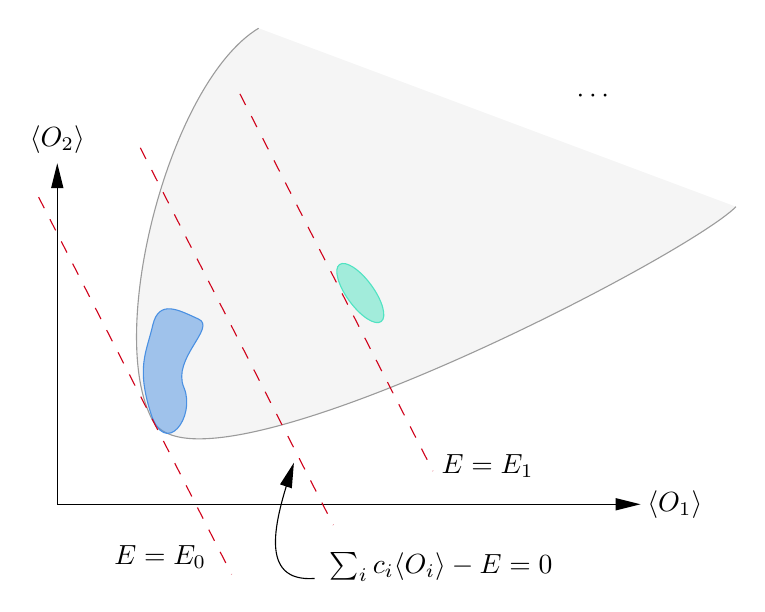
\begin{tikzpicture}[x=0.75pt,y=0.75pt,yscale=-1,xscale=1]
%uncomment if require: \path (0,353); %set diagram left start at 0, and has height of 353

%Curve Lines [id:da34254251114708456] 
\draw [color={rgb, 255:red, 155; green, 155; blue, 155 }  ,draw opacity=1 ][fill={rgb, 255:red, 155; green, 155; blue, 155 }  ,fill opacity=0.1 ]   (274,16.64) .. controls (231,42.64) and (200,163.64) .. (223,205.64) .. controls (246,247.64) and (479,127.64) .. (504,102.64) ;
%Straight Lines [id:da904255078328454] 
\draw    (177,246) -- (456,246) ;
\draw [shift={(458,246)}, rotate = 180] [fill={rgb, 255:red, 0; green, 0; blue, 0 }  ][line width=0.08]  [draw opacity=0] (12,-3) -- (0,0) -- (12,3) -- cycle    ;
%Straight Lines [id:da28860077544833507] 
\draw    (177,246) -- (177,83.73) ;
\draw [shift={(177,81.73)}, rotate = 90] [fill={rgb, 255:red, 0; green, 0; blue, 0 }  ][line width=0.08]  [draw opacity=0] (12,-3) -- (0,0) -- (12,3) -- cycle    ;
%Shape: Polygon Curved [id:ds05129166801576668] 
\draw  [color={rgb, 255:red, 74; green, 144; blue, 226 }  ,draw opacity=1 ][fill={rgb, 255:red, 74; green, 144; blue, 226 }  ,fill opacity=0.5 ] (223,159.73) .. controls (226,146.73) and (236,152.73) .. (245,156.73) .. controls (254,160.73) and (232,175.73) .. (238,189.73) .. controls (244,203.73) and (229,224.27) .. (222,202) .. controls (215,179.73) and (220,172.73) .. (223,159.73) -- cycle ;
%Straight Lines [id:da6483527344854445] 
\draw [color={rgb, 255:red, 208; green, 2; blue, 27 }  ,draw opacity=1 ] [dash pattern={on 4.5pt off 4.5pt}]  (168,98) -- (261,279.73) ;
%Straight Lines [id:da0036541181567224523] 
\draw [color={rgb, 255:red, 208; green, 2; blue, 27 }  ,draw opacity=1 ] [dash pattern={on 4.5pt off 4.5pt}]  (217,74.27) -- (310,256) ;
%Straight Lines [id:da34767057063343554] 
\draw [color={rgb, 255:red, 208; green, 2; blue, 27 }  ,draw opacity=1 ] [dash pattern={on 4.5pt off 4.5pt}]  (265,48.27) -- (358,230) ;
%Shape: Ellipse [id:dp302165402812995] 
\draw  [color={rgb, 255:red, 80; green, 227; blue, 194 }  ,draw opacity=1 ][fill={rgb, 255:red, 80; green, 227; blue, 194 }  ,fill opacity=0.5 ] (312.97,130.5) .. controls (310.07,132.62) and (312.21,140.48) .. (317.75,148.06) .. controls (323.29,155.64) and (330.13,160.08) .. (333.03,157.96) .. controls (335.93,155.84) and (333.79,147.98) .. (328.25,140.4) .. controls (322.71,132.81) and (315.87,128.38) .. (312.97,130.5) -- cycle ;
%Curve Lines [id:da7414078371933952] 
\draw    (301,281.73) .. controls (273.56,283.69) and (281.65,253.87) .. (290.46,227.6) ;
\draw [shift={(291,226)}, rotate = 108.67] [fill={rgb, 255:red, 0; green, 0; blue, 0 }  ][line width=0.08]  [draw opacity=0] (12,-3) -- (0,0) -- (12,3) -- cycle    ;

% Text Node
\draw (460,246) node [anchor=west] [inner sep=0.75pt]    {$\langle O_{1} \rangle $};
% Text Node
\draw (177,78.33) node [anchor=south] [inner sep=0.75pt]    {$\langle O_{2} \rangle $};
% Text Node
\draw (307,268) node [anchor=north west][inner sep=0.75pt]    {$\sum _{i} c_{i} \langle O_{i} \rangle -E=0$};
% Text Node
\draw (250,264.73) node [anchor=north east] [inner sep=0.75pt]   [align=left] {$\displaystyle E=E_{0}$};
% Text Node
\draw (360.97,234.5) node [anchor=south west] [inner sep=0.75pt]   [align=left] {\textcolor[rgb]{0,0,0}{$\displaystyle E=E_{1}$}};
% Text Node
\draw (426,45.4) node [anchor=north west][inner sep=0.75pt]    {$\cdots $};


\end{tikzpicture}

    \caption{线性SDP和非线性SDP:蓝色和绿色区域是非线性SDP的可行域,蓝色区域近似给出基态$E_0$上的物理量期望值,绿色区域近似给出基态$E_1$上的物理量期望值,灰色区域是线性SDP问题的可行域,虚线代表不同$E$对应的$\sum_i c_i \expval{O_i} = E$超平面,其中$c_i$为哈密顿量$H = \sum_i c_i O_i$的系数。}
    \label{fig:feasibility-compare}
\end{figure}

虽然非线性SDP能够让我们看清楚系统的激发态结构,目前尚无足够成熟的非线性求解器能够求解物理上需要的非线性SDP问题\cite{kazakov2021analytic}。
已报道的非线性SDP均仅限于单粒子量子力学,通过递推关系,将所有物理量约化至$E$和$\expval*{x^2}$上,然后暴力搜索\cite{han_matrix,bhattacharya2021}。
我们将在\prettyref{sec:nonlinear-sdp-oscillator}中复现\parencite{han_matrix}的工作。

\subsection{数值bootstrap的若干应用}

由于bootstrap不依赖于哈密顿量中各项的大小,它显然是处理非微扰问题的有力武器。
已有若干关于不同体系的数值bootstrap研究出现,如关于难以微扰解决的单粒子量子力学问题和矩阵模型\cite{han_matrix,bhattacharya2021,kazakov2021analytic}以及强关联电子模型\cite{han_manybody}。

文献\parencite{bhattacharya2021}使用了以$E$和$\expval*{x^2}$为优化变量、暴力搜索的单粒子量子力学非线性SDP,捕捉到了二势阱模型中的非微扰瞬子效应,并与通过稀薄瞬子假设计算出的基态能量比较,直观展示了稀薄瞬子假设的成立条件;验证了互为对偶的超对称量子力学哈密顿量的谱的确是一致的;验证了$O(N)$向量模型的低能部分在强耦合极限下,基态能量和耦合常数的分数幂次关系,并确认其与解析结果一致。
\parencite{kazakov2021analytic}开发了一套处理矩阵模型的数值bootstrap中的矩阵自由度在大$N$极限下满足的非线性约束
\begin{equation}
    \left\langle\operatorname{Tr} M^{l} \operatorname{Tr} M^{m}\right\rangle=\left\langle\operatorname{Tr} M^{l}\right\rangle\left\langle\operatorname{Tr} M^{m}\right\rangle+\mathcal{O}\left(1 / N^{2}\right)
\end{equation}
的方法,验证了它在求解可以解析处理的矩阵模型时的有效性,并借此解决了无法解析处理的一类二矩阵矩阵模型。%
\footnote{这套方法对非线性SDP的作用可能有限,因为此时\eqref{eq:nonlinear-energy}和\eqref{eq:target-function}联立将导致任意高幂次的非线性约束,而矩阵模型中由于矩阵自由度的非线性约束幂次最多到2。}%
文献\parencite{han_manybody}将线性SDP数值boostrap技术应用在一维和二维Hubbard模型上,所得结果和常规的DQMC、DMRG等方法吻合。

\section{关于本文}

本文将探讨

\chapter{一维非线性谐振子的数值bootstrap}

\section{一维非线性谐振子——一个$0+1$维非微扰场论}

一维非线性谐振子
\begin{equation}
    H = p^2 + x^2 + g x^4
\end{equation}
可以看成一个$0+1$维的$\phi^4$量子场论。它常常被用作量子力学中微扰论的例子,但实际上可以证明,其基态能量的微扰级数是发散的\cite{PhysRev.184.1231}。
这个发散可以看成$\phi^4$量子场论中的发散的一个特例。大部分量子场论中,相互作用均导致的微扰级数在最好的情况下也是渐进级数\cite{Jackiw_effective}。%
\footnote{此处所说的是朴素地将物理量展开成关于耦合常数$g$的幂次的级数后,会发现这个级数不收敛。在量子场论中这个级数的每一项都可能不收敛,因为动量积分时发生紫外发散。后一种不收敛和此处的讨论没有直接关系。然而,\emph{重整化微扰论}——在微扰级数中引入抵消项,物理地看,是使用修饰后的耦合常数取代裸的耦合常数——可以用于消除紫外发散,而重整化微扰论的收敛性确实在\parencite{Bender-1970uz}中讨论过,结论是,很不幸,它仍然是发散的。}

由于一维非线性谐振子归根到底是一个量子力学模型,可以通过求解离散定态薛定谔方程的方法精确地处理它。
它和$3+1$维多体问题的相似性又意味着,用于一般的多体问题的方法也可以用在它上面。
一维非线性谐振子的简单形式和它的非微扰本质意味着它是测试多体问题研究方法的一个理想的玩具模型:可以通过比较这些数值或是解析方法和求解离散定态薛定谔方程的结果来预计这些方法的有效性,并分析这些方法为何有效或无效。
一维非线性谐振子已被做大量不同的话题的例子,包括泛函重整化群\cite{Nagy-2010fv}、Rayleigh-Schrödinger微扰论的高阶行为\cite{bender199041}、重整化微扰论的收敛性\cite{Bender-1970uz}、量子多尺度分析\cite{Bender_1996}。

之后几节将重复

\section{非线性SDP优化}\label{sec:nonlinear-sdp-oscillator}

\subsection{$\expval{x^n}$的非线性递推关系}

\subsection{可行域,基态和第一激发态}

\subsection{严格对角化基准测试}

\subsection{非线性SDP在大规模问题上的不可行性}

\section{线性SDP优化}

\subsection{对易子和等式关系的符号计算}

\subsection{构建优化问题}

\subsection{使用非线性SDP为线性SDP做基准测试}

\subsection{收敛性问题}

\chapter{Hubbard模型的数值bootstrap}

\section{一维Hubbard模型的数值bootstrap}

\subsection{算符空间的选取和截断}

\subsection{等式约束和半正定约束的符号计算}

\subsection{DMRG基准测试}

\section{二维Hubbard模型的数值bootstrap}

\chapter{总结与展望}


% 后置部分包含参考文献、声明页(自动生成)等
\backmatter

% 打印参考文献列表
\printbibliography

\chapter{致\quad 谢}

\chapter{附\quad 录}

\end{document}
